 \subsubsection{UC10 - Home}
  \begin{figure}[H]
 	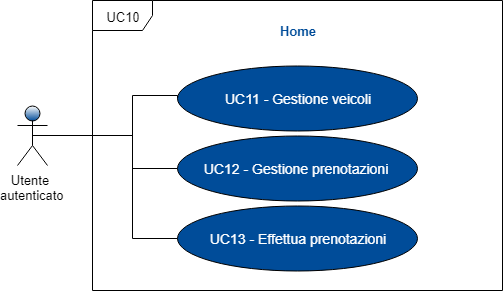
\includegraphics[width=10cm]{res/images/UC10-Home.png}
 	\centering
 	\caption{UC10 - Home}
 \end{figure}
 \begin{itemize}
 	\item \textbf{Attori Primari}: utente autenticato;
 	\item \textbf{Descrizione}: l'utente ha una panoramica di quello che può fare nel momento in cui accede all'applicazione, infatti, ha la possibilità di ricercare un veicolo con cui viaggiare ed effettuare quindi una prenotazione, gestire i propri veicoli oppure visualizzare le prenotazioni attive al momento;
 	\item \textbf{Scenario principale}: l'utente autenticato, dopo l'accesso, viene portato nella sezione "viaggia" in cui ha la possibilità di:
 	\begin{itemize}
 		\item ricercare un veicolo ed effettuare una prenotazione [UC13];
 		\item gestire i propri veicoli [UC11].
 	\end{itemize}
 	\item \textbf{Scenario alternativo}: l'utente autenticato, dopo l'accesso, cambia sezione ed entra nelle "prenotazioni" in cui ha la possibilità di:
	 	\begin{itemize}
	 		\item visualizzare le prenotazioni attive [UC12]. 
	 	\end{itemize}
 	\item \textbf{Precondizione}: l'utente accede al fragment\glosp della \textit{Home} dopo aver fatto l'accesso all'applicazione;
 	\item \textbf{Postcondizione}: l'utente decide di accedere ad una delle due sezioni messa a disposizione.
 \end{itemize}